\documentclass[twocolumn]{article}
\usepackage{graphicx}
\usepackage[utf8]{inputenc}
\usepackage[a4paper, margin=0.79in]{geometry}
\usepackage{lastpage}
\usepackage[compact]{titlesec}

\titleformat{\section}[hang]{\bfseries\large}{\thesection}{0.5em}{}
\titleformat{\subsection}[hang]{\bfseries\normalsize}{\thesubsection}{0.5em}{}
\titleformat{\subsubsection}[runin]{\bfseries\normalsize}{\thesubsubsection}{0.5em}{}

\title{\large{\textbf{ACS Lab 1 - Matrix Multiplication}}}
\author{
    \small Chris Wouters (, chriswouters)
    \and \small Lonnie Donaho (student nr, netid)
    \and \small Another Name (student nr, netid)
}
\date{}

\begin{document}

\maketitle

\begin{center}
    \footnotesize{Report contains \pageref{LastPage} of maximum 6 pages.}
\end{center}

\section{Introduction}
Briefly describe what you are going to show in this report, which benchmarks.

\section{Experimental setup}
\textsc{Briefly describe the systems you have benchmarked on, and by which methods you have measured.}


This first assignment consists in the implementation of a matrix multiplication functions with C++ with different methods: using SIMD instructions, on multiple cores with OpenMP and on a GPU using OpenCL.

Once implemented  and  optimized them, a comparison between the different implementations  will be done, analyzing the performance  and the suitability of each method for the  matrix multiplication of  different sizes.


\section{Vector inner product}
\subsection{Description}
\textsc{Briefly describe this benchmark.}

The vector inner product can be obtained by multiplying two matrices of the one row and column.
From the experiments.hpp file the vector inner product will be performed and the results will be stored in vec.csv file.

\subsection{Profile}
Briefly describe and show graphs of the performance of your baseline implementation.
\begin{figure}[h]
    \centering
    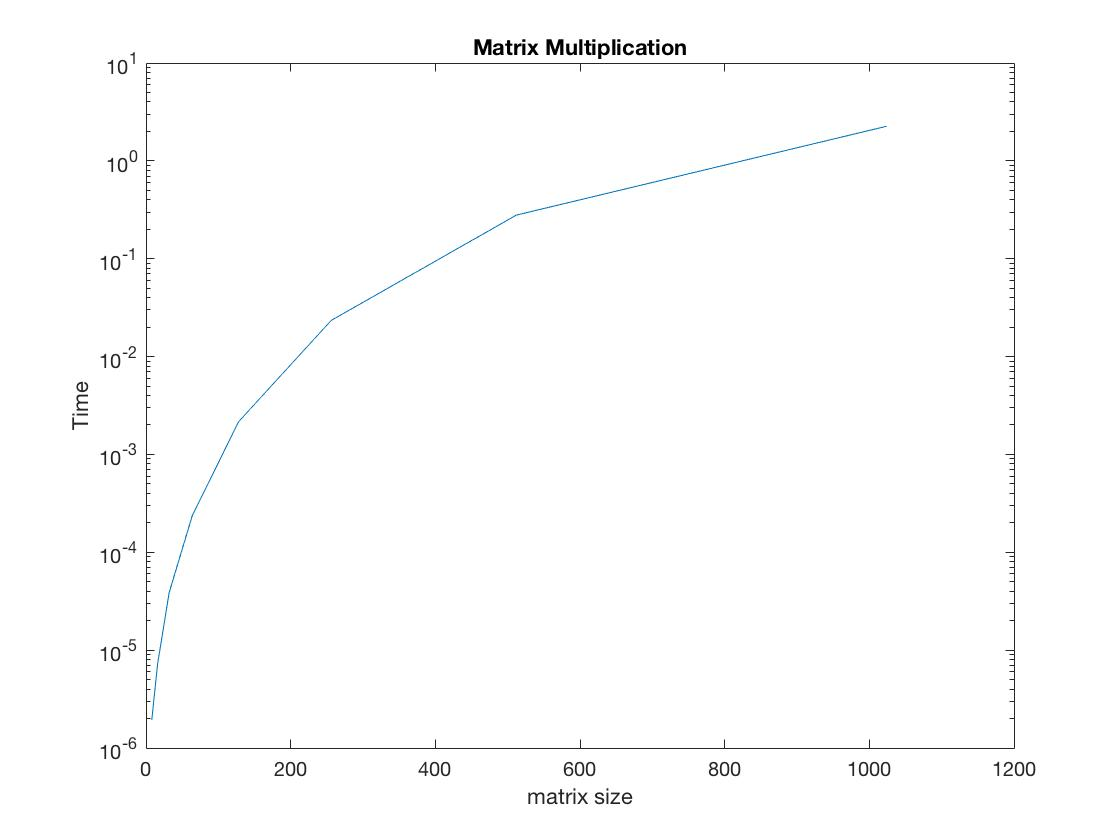
\includegraphics[width=0.45\textwidth]{matrix_mult.jpg}
    \caption{Matrix Multiplication}
    \label{fig:OpenMP_base}
\end{figure}
\subsection{Discussion}
Briefly discuss / conclude peculiarities about this benchmark.

\section{Matrix multiplication}
\subsection{Description}
\textsc{Briefly describe this benchmark.}
The matrix multiplication benchmark is described in the experiments.hpp file provided. 
In the matrix file provided by the source code a function that test the feasibility and result of a multiplication of two matrices is already implemented.
The main matrix-multiplication function  receives two matrices as arguments and after testing if it is possible to multiply them  the function proceeds to obtain the resulting matrix.
The procedure  followed by this function consists on three for loops where the dot product of each row of the first matrix and each column of the second one is calculated and stored in the corresponding  place of the output matrix.
The resulted matrix is stored in the file mat.csv.

\subsection{Estimation}

Briefly describe an estimation about the performance of matrix multiplication w.r.t. the vector baseline benchmark.
\subsection{Profile}
Briefly describe and show graphs of the performance of your baseline implementation.
\subsection{Discussion}
Briefly discuss / conclude peculiarities about this benchmark.

\section{SIMD extensions}
\subsection{Description}
Briefly describe this benchmark.
\subsection{Profile}
Briefly describe and show graphs of the performance of your baseline implementation.
\subsection{Estimation}
Briefly describe what improvements you can make based on the profile, and how much benefit it will give (in terms of e.g. speedup, throughput).
\subsection{Design and implementation}
Briefly describe all discrete improvements that you've made.
\subsubsection{Improvement X}
Your description goes here.
\subsubsection{Improvement Y}
\subsection{Results after improvement}
Briefly show the results after improvements.
\subsubsection{Results after improvement X}
\subsubsection{Results after improvement Y}
\subsection{Discussion}
Briefly discuss / conclude your work on this benchmark.

\section{OpenMP}
\subsection{Description}
The OpenMP benchmark is based on the execution of the matrix multiplication function in parallel. The number of threads are chosen by the user and the parallel part of the code will determine the performance of the system.

\subsection{Profile}
The  OpenMP function is evaluated by means of time depending on the size of the matrix and the number of threads.
The baseline function results confirm the Amdahl's law. 
\begin{figure}[h]
    \centering
    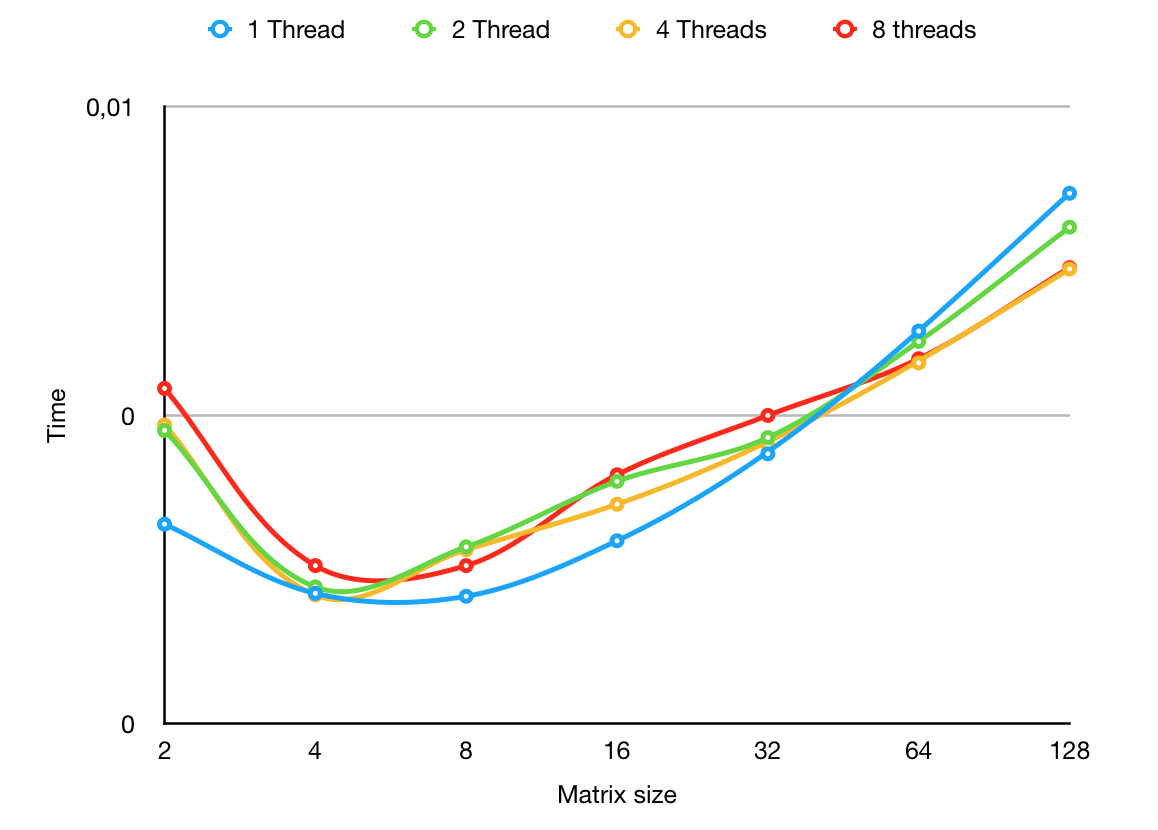
\includegraphics[width=0.45\textwidth]{OpenMP_bas.png}
    \caption{Caption}
    \label{fig:OpenMP_base}
\end{figure}

In  Figure \ref{fig:OpenMP_base} the result of the baseline OpenMP time for the different sizes of the matrix is depicted. For small matrices the performance improvement of the parallel code is negligible due to the reduction of the time executing in parallel  the for loops is compensated by time spent during the division of the work among the threads. However, if the resulting matrix is bigger than 64x64 the parallelism of the function improves the performance considerably. 


\subsection{Estimation}
Based on Amdahl's Law the speedup of the system can be calculated knowing the percentage of the parallel tasks.
In the first version of the Open MP code only on of the two main for loops  is parallelized, considering that it is approximately 50\% code, the expected speedup of the system is  1,33.
As explained briefly before, the system throughput is benefited from the parallelism when the matrix size is big.

\subsection{Design and implementation}
\textsc{Briefly describe all discrete improvements that you've made.}

The portion of code that is parallelized will determine the performance of the system.
With the main objective of reducing the time spent during the matrix multiplication function the parallel portion of code is maximize.


\subsubsection{Improvement X}
\subsubsection{Improvement Y}
\subsection{Results after improvement}
Briefly show the results after improvements.
\subsubsection{Results after improvement X}


\subsubsection{Results after improvement Y}
\subsection{Discussion}
Briefly discuss / conclude your work on this benchmark.

\section{OpenCL}
\subsection{Description}
Briefly describe this benchmark.
\subsection{Profile}
Briefly describe and show graphs of the performance of your baseline implementation.
\subsection{Estimation}
Briefly describe what improvements you can make based on the profile, and how much benefit it will give (in terms of e.g. speedup, throughput).
\subsection{Design and implementation}
Briefly describe all discrete improvements that you've made.
\subsubsection{Improvement X}
\subsubsection{Improvement Y}
\subsection{Results after improvement}
Briefly show the results after improvements.
\subsubsection{Results after improvement X}
\subsubsection{Results after improvement Y}
\subsection{Discussion}
Briefly discuss / conclude your work on this benchmark.

\section{Conclusion}

\begin{thebibliography}{}
\bibitem{SomeReference} 
Some Author
\textit{Some Title}
Some Information about how to find this reference.
\end{thebibliography}

\end{document}
